\chapter{TGC検出器のタイミング較正}
\thispagestyle{empty}
\label{chap:5}
LHC-ATLAS~実験において、信号のタイミング調整は適切にミューオンを捉えるために非常に重要である。40~MHz(ビーム衝突間隔~25~ns)~という高頻度の陽子衝突から生成されるミューオン等の荷電粒子を捉えるには、ゲート幅の調整や詳細な遅延パラメータの設定が鍵を握る。
\chapref{chap:4}で述べた通り、TGC~検出器では粒子信号の読み取りを適切に行うために、複数の遅延回路が実装されている。
本章では、モンテカルロシミュレーションおよび~2018~年の~Run~2~実験データを用いて、TGC~検出器のタイミングに関する調査を行い、TGC~エレクトロニクスの設定検証を行う。
TGC~検出器における詳細なタイミング設定に関する理解を深め、Run~3~に向けた性能改善を提案する。

\section{バンチ判定の比較}
本節では、TGC~検出器での測定において得られたバンチ判定の分布およびトリガー判定について説明する。

先行研究において~TGC~がトリガーを発行するタイミングについての研究が行われている~\cite{MT:05}。2011~年、LHC~では~50~ns~間隔(20~MHz)の陽子バンチ衝突での運転を行った。通常~LHC~クロックは~1~周期~25~ns~なので、50~ns~間隔でのバンチ衝突の場合はクロック~2~周期ごとにバンチ衝突が起こることになる。したがって、2~周期のうち~1~周期分はバンチ衝突が起こらず、トリガーが発行されないような設定となっている。\subsecref{subsec:l1tri}で説明したように、L1~トリガーはパイプライントリガーである。よって、以上の設定においてトリガー判定を正しく行うには、前のバンチおよび次のバンチでバンチ衝突が起こらないため、基準バンチのタイミングが正しく調整されている必要がある。先行研究では、上記の運転におけるデータから~TGC~におけるトリガー判定のタイミングの評価を行った。結果としては、前のバンチと判定されて失う事象はないこと、SL~におけるコインシデンスは、前かつ基準バンチ、基準バンチ、基準かつ次のバンチで得られる可能性があり、前かつ基準バンチでの信号を得る確率は~$10^{-4}$~ほどの無視できる割合であることが示された。

\figref{fig:bcid00}に、Run~2~実験データおよびシミュレーションにおけるバンチ判定の分布の一例を示した。バンチ判定は、\subsubsecref{subsubsec:bcid}で示したように、前のバンチ、前かつ基準バンチ、基準バンチ、基準かつ次のバンチで識別される。シミュレーションと実験データの分布を比較すると、実験データの方がタイミングの揺らぎが大きく、特に基準かつ次のバンチの割合が高いことがわかる。基準かつ次のバンチの割合が多ければ、非効率な損失が起こることも懸念される。Run~3~の開始に向けて、トリガー判定を損失なく正確に行うには、より詳細なバンチ判定における議論が必要となる。また\secref{sec:latemu}で述べたように次のバンチと判定される粒子も新物理探索において重要なファクターとなり、基準バンチのタイミングが正しく調整されていなければ、次のバンチで測定される粒子の速度にもばらつきが生じることが考えられる。よって、本研究ではシミュレーションを用いて~TGC~検出器の詳細なタイミング較正を行う。

\begin{figure}[H]
        \centering   
        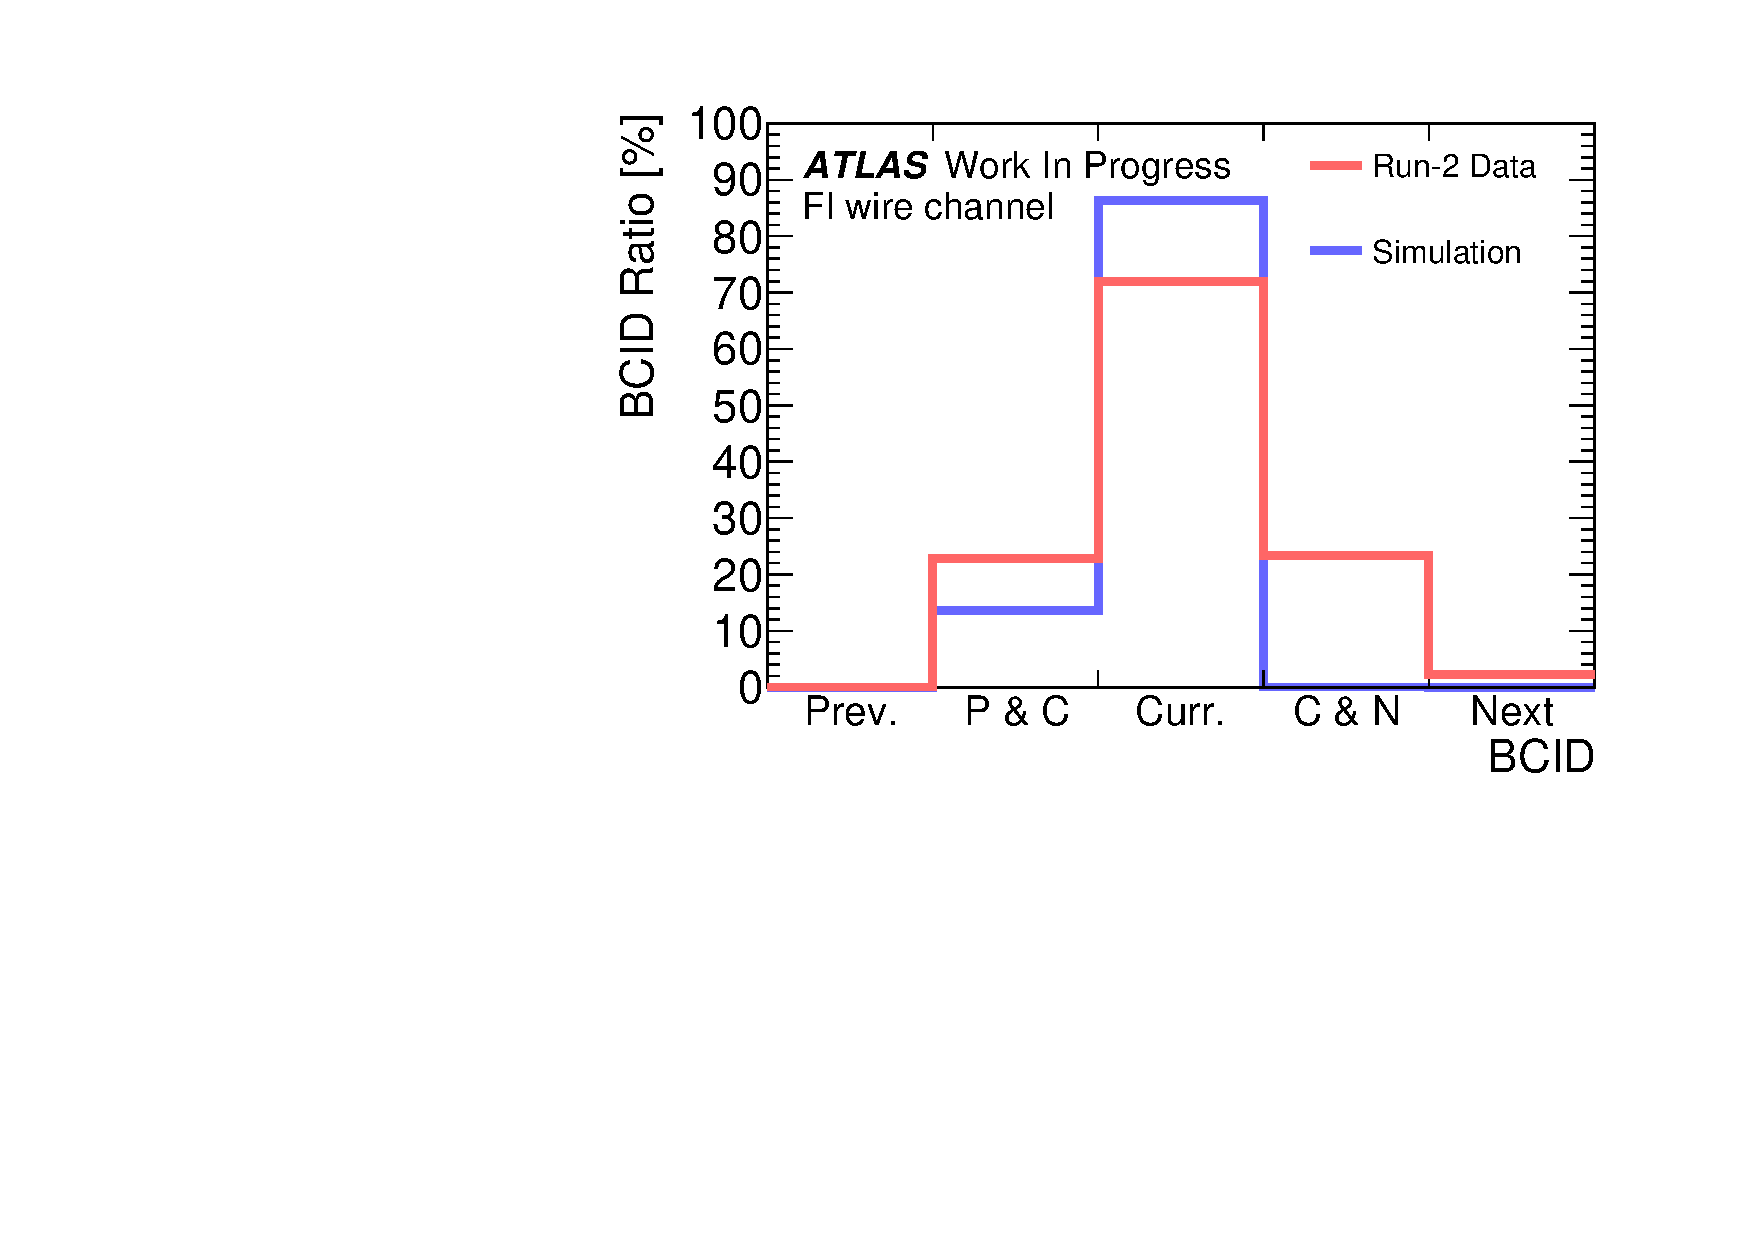
\includegraphics[width=0.75\textwidth,page=1]{img/pdf5/BCID0.pdf}
        \caption[Run~2~実験データとモンテカルロシミュレーションにおけるバンチ判定の分布]{Run~2~実験データとモンテカルロシミュレーションにおけるバンチ判定の分布。FI~T10~チェンバー、wire~チャンネル。}
        \label{fig:bcid00}
\end{figure}

\section{解析のデータサンプル}
研究に用いた解析のデータサンプルについて説明する。

\subsection{Run~2~実験データ}
本研究では~Run~2~の実験データとして~2018~年に行われた~Run~2~period~B~の実験データを使用した。
統計量としては、約~400~万事象である。
2018~年には~period~A~-~period~R~までの運転が行われている。

\subsection{モンテカルロシミュレーション}
シミュレーションに関しては統計量の確保のため、シングルミューオンサンプルを使用した。$3~\rm{GeV}~<~p_{\rm{T}}~<~80~GeV$~の範囲の横運動量を持つミューオンのサンプルとなっている。統計量としては約~50~万事象である。

ATLAS~実験におけるイベントシミュレーションは、Athena~\cite{URL:21}~と呼ばれるソフトウェアチェーンを用いて行われる。Athena~では複数の段階に分けてデータ処理が行われ、最終的に実験データと同様の解析が行えるように処理されていく。以下では、それぞれの段階におけるシミュレーションの詳細について述べる。

\subsubsection{イベント生成(Generation)}
物理事象そのもののシミュレーションを行う。様々なイベントジェネレータが利用されている。

\subsubsection{検出器シミュレーション(Simulation)}
生成イベントの粒子の検出器中での振る舞い(物質との反応や粒子の崩壊など)を~Geant4~\cite{URL:22}や簡易シミュレーター~Atlfast-II~\cite{TR:08}を用いてシミュレートする。この段階では物質を通過した時刻、場所とそこで落とされたエネルギー損失がデータとして保持される。この状態のデータフォーマットは~Hit~と呼ばれる。

\subsubsection{デジタイゼーション(Digitization)}
Hit~データを元に、検出器の信号をシミュレーションを行う。通過時刻、場所とエネルギー損失から信号の発生時間や大きさなどを計算する。その結果はDigitと呼ばれている。Digit~は同等の情報を含むデータフォーマット~RDO(Raw~Data~Object)に変換される。Byte~Stream~と呼ばれる実データもRDOに変換され、情報処理が行われる。

\subsubsection{再構成(Reconstruction)}
RDO~を元にトラックやクラスターを再構成し粒子識別を行う。
その結果を~ESD(Event~Summary~Data)として保存する。実際には解析のための物理情報を集約した~AOD(Analysis~Object~Data)も同時に生成している。

\subsubsection{解析(Analysis)}
ESD~や~AOD~を元に、ROOT~\cite{URL:23}~で扱える~ntuple(ROOTではTTreeと呼ばれる)やヒストグラムを生成を行う。

\section{TGC~デジタイゼーション}
モンテカルロシミュレーションの~TGC~デジタイゼーションでは、実験におけるバンチ交差識別を再現するために~TGC~検出器内での反応の様々なシミュレーション処理が行われている。ここでは、本研究以前のシミュレーションにおける信号伝搬や遅延等の計算について述べる。シミュレーションにおける信号伝搬の計算について以下にまとめた。

\begin{itemize}
\item 信号伝搬に伴う時間
\begin{itemize}
\item time of flight:衝突点から各 TGC に到達するまでの時間。
\item time jitter:センサーに信号が検出されるまでの時間。
\item propagation time:wire および strip において信号が伝播する時間。
\end{itemize}
\end{itemize}
\begin{itemize}
\item 信号遅延
\begin{itemize}
\item tof correction:time of flight による遅延を吸収するための時間。
\item time offset:信号遅延時間の補正。
\end{itemize}
\end{itemize}

シミュレーションにおいては粒子の生成から信号検出までの伝搬時間を計算している。また信号遅延では、検出までの時間差を吸収するための計算が行われている。すなわち、以下の\equref{eq:tdigit}で表される時間~$\rm{T_{Digit}}$~と~BCID~ゲートを比較することでバンチ交差識別を行う。

\begin{align}
    \it{T_{\rm{Digit}}=T_{\rm{timeOfFlight}}+T_{\rm{jitter}}+T_{\rm{propagation}}-T_{\rm{tofCorrection}}-T_{\rm{timeOffset}}}
    \label{eq:tdigit}
\end{align}

\section{TGC~検出器のタイミング較正}
Run~2~の実験データ、モンテカルロシミュレーションにおけるタイミングの評価を行う。Run~2~の実験データをより詳細に再現し、シミュレーションのタイミング較正を行うことで実験データとの差異を削減し、より不定性の少ないシミュレーションの実装を目指す。本節では、TGC~検出器のタイミング較正の結果について示す。

\subsection{解析手法}
実験データおよびシミュレーションサンプルの解析手法について説明する。
Run~2~の実験データにおいては、トリガーを通過した粒子の情報のみが保存されているため、バイアスがかかり物理解析に影響が及ぶ可能性がある。そこで解析の手法として~Tag~and~Probe~法を用いる。本研究では、$Z$ボソン由来のミューオン候補を用いる。一回のバンチ衝突に対し、2~つ以上のミューオン候補が存在するイベントを選択する。それらのミューオン候補のうち、電荷が異符号となっているミューオンペアを選び出し、不変質量を再構成する。再構成の条件は、$81~\rm{GeV}~<~M_{Z}~<~101~\rm{GeV}$~としている。選択されたミューオンペアは~$Z$ボソン由来であり、正しく再構成されたミューオンであるということが保証される。この~2~つのミューオンのうち、一方を~Tag~ミューオンとする。続いて~Tag~ミューオンがトリガーを通過したかどうかを判定する。トリガー判定には、HLT~の標準的なシングルミューオントリガーである~$\rm{HLT\_mu26\_ivarmeduium}$~を利用する。ここでトリガー通過の判定のために~$\Delta~R=\sqrt{(\Delta~\eta)^2+(\Delta~\phi)^2}$を定義する。ここで~$\Delta~\eta$,~$\Delta~\phi$~はそれぞれ~トリガーが発行された飛跡と~Tag~ミューオンにおける~$\eta$~方向、$\phi$~方向の差である。$\Delta~R~<~0.001$~を満たせば~Tag~ミューオンがトリガーを発行したとみなす。このとき、もう一方のミューオンはバイアスを受けずに使用することができる。このミューオンを~Probe~ミューオンと呼び、解析に使用する。

\subsection{バンチ判定の分布とタイミングの評価方法}
バンチ判定は各チャンネルでの入力信号毎に行われる。したがって各~TGC~の各チャンネル毎のバンチ判定の事象数をもとにタイミングの評価を行う。タイミングの評価のために以下のようなパラメータを用いた。
\begin{align}
    \it{P_{\rm{Timing}}}=\frac{\it{N_{\rm{Curr.}}}×\rm{0}+\it{N_{\rm{Curr.\&Next}}}×\rm{0.5}+\it{N_{\rm{Next}}}×\rm{1}}{\it{N_{\rm{Curr.}}}~+~\it{N_{\rm{Curr.\&Next}}}~+~\it{N_{\rm{Next}}}} \label{eq:timing}
\end{align}
$\it{N_{\rm{Curr.}}}$,~$\it{N_{\rm{Curr.\&Next}}}$,~$\it{N_{\rm{Next}}}$~~はそれぞれ基準バンチ、基準かつ次のバンチ、次のバンチの事象数を表している。
\equref{eq:timing}を用いることで、基準バンチに対してどれだけタイミングが遅れているかを評価することができる。\figref{fig:timingex}に一例を示した。プロット点が~0~付近に位置しているほど、基準バンチで判定されている割合が多く理想的な状態であると言える。反対に、基準かつ次のバンチ、次にバンチの割合が多くなるほどパラメータの数値が大きくなり、タイミングの遅れが最大となるとプロット点が~1~となる。

\begin{figure}[H]
        \centering   
        \includegraphics[width=0.75\textwidth,page=21]{img/pdf5/master_timingplot_data.pdf}
        \caption[タイミングパラメータを用いた TGC 検出器の評価]{タイミングパラメータを用いた TGC 検出器の評価。M2~T08~チェンバー、strip~チャンネル。数値が高いほど、タイミングが遅れていることを表す。}
        \label{fig:timingex}
\end{figure}

\subsection{モンテカルロシミュレーションの改良}
\label{sec:imp}
シミュレーションと実験における信号伝搬に関して比較を行うと、シミュレーションにおいて計算の実装が不十分な点が示唆された。以下ではシミュレーションにおける問題点を明らかにしシミュレーションの改良を行なった点について述べる。

\subsubsection{センサーから~ASD~までの信号伝搬の計算}
wire~および~strip~で信号が伝搬するのち~ASD~で信号が検出されるまでには、センサー(wire,~strip)の端からチェンバーに沿って~ASD~に到達するまでの時間を考慮する必要がある。しかし、シミュレーションにおいてはタイミングに大きな影響はないと考えられ計算の実装が行われていなかった。したがってシミュレーションに新たに~ASD~の位置座標の情報を追加し伝搬時間の計算を実装した。
\figref{fig:asd}に示したのは、ASD~までの信号伝搬時間を計算に実装した前後によるシミュレーションの比較である。ASD~までの伝搬時間を考慮したことにより、ASD~の位置から離れるほどタイミングに遅れが生じていることがわかる。

\begin{figure}[H]
    \begin{minipage}{0.49\hsize}
    \centering   
    \includegraphics[width=\textwidth,page=8]{img/plot/ASD.pdf}
    \subcaption{}
    \end{minipage}
    \begin{minipage}{0.49\hsize}
    \centering   
    \includegraphics[width=\textwidth,page=35]{img/plot/ASD.pdf}
    \subcaption{}
    \end{minipage}
    \caption[センサーから~ASD~までの伝搬時間の実装によるタイミングの評価]{センサーから~ASD~までの伝搬時間の実装によるタイミングの評価。青は、ASD~までの信号伝搬が未実装、赤は、ASD~までの信号伝搬が実装されたシミュレーションを表す。(a)~M1~T7~チェンバー、wire~チャンネル。(b)~M3~T9~チェンバー、strip~チャンネル。}
    \label{fig:asd}
\end{figure}

\subsubsection{EIFI~におけるツイストケーブルの半径に依存した遅延時間の計算}
センサーからの信号の出力はシグナルケーブルにまとめられ~ASD~まで伝搬される。シグナルケーブルは40~対のツイストケーブルで、断面図を見ると二重構造となっており、内側と外側で経路差が生じる~\cite{MT:04}。\figref{fig:twist0}にシグナルケーブルの断面の概念図を示す。また\figref{fig:twist00}は実際に使用されたシグナルケーブルの写真である。センサーにおける~32~チャンネルのうち~12-16~チャンネルおよび~27-32~チャンネルはケーブルの内側に配置されている。内側と外側のチャンネルの伝搬時間差はケーブル長に対して1~$\%$~程度と見積もられている。EIFI~に関しては、構造上~BW~と比べてケーブル長が大きく(BW:2.8~-~12.5~m,~EIFI:26.9~-~46.1~m)、セクター毎の長さの差も大きい。1~m~あたり~5~ns~で信号が伝搬すると考えれば、最大で約0.4~m(約2~ns)の差が生じる。よって、セクター毎のケーブル長とケーブルの内側と外側における経路差の影響による遅延時間の計算をシミュレーションに新しく実装した。

\figref{fig:twist}は、ツイストケーブルの影響を計算に実装する前後のタイミングを比較したものである。実装以前は位置に依存した一定のタイミング変化になっているが、実装を行ったことにより~11~チャンネルと~12~チャンネルおよび~26~チャンネルと~27~チャンネルの間に大きなタイミングの変化があることがわかる。

\begin{figure}[H]
    \centering   
    \includegraphics[width=0.8\textwidth,page=6]{img/slide/slide.pdf}
    \caption[シグナルケーブルの断面の概念図]{シグナルケーブルの断面の概念図~\cite{MT:04}。一つ一つの信号線はねじれるようにまとめられている。1-11~ch~および~17-26~ch~は断面の外側、12-16~ch~および~27-32~ch~は断面の内側に配置されている。}
    \label{fig:twist0}
\end{figure}

\begin{figure}[H]
    \centering   
    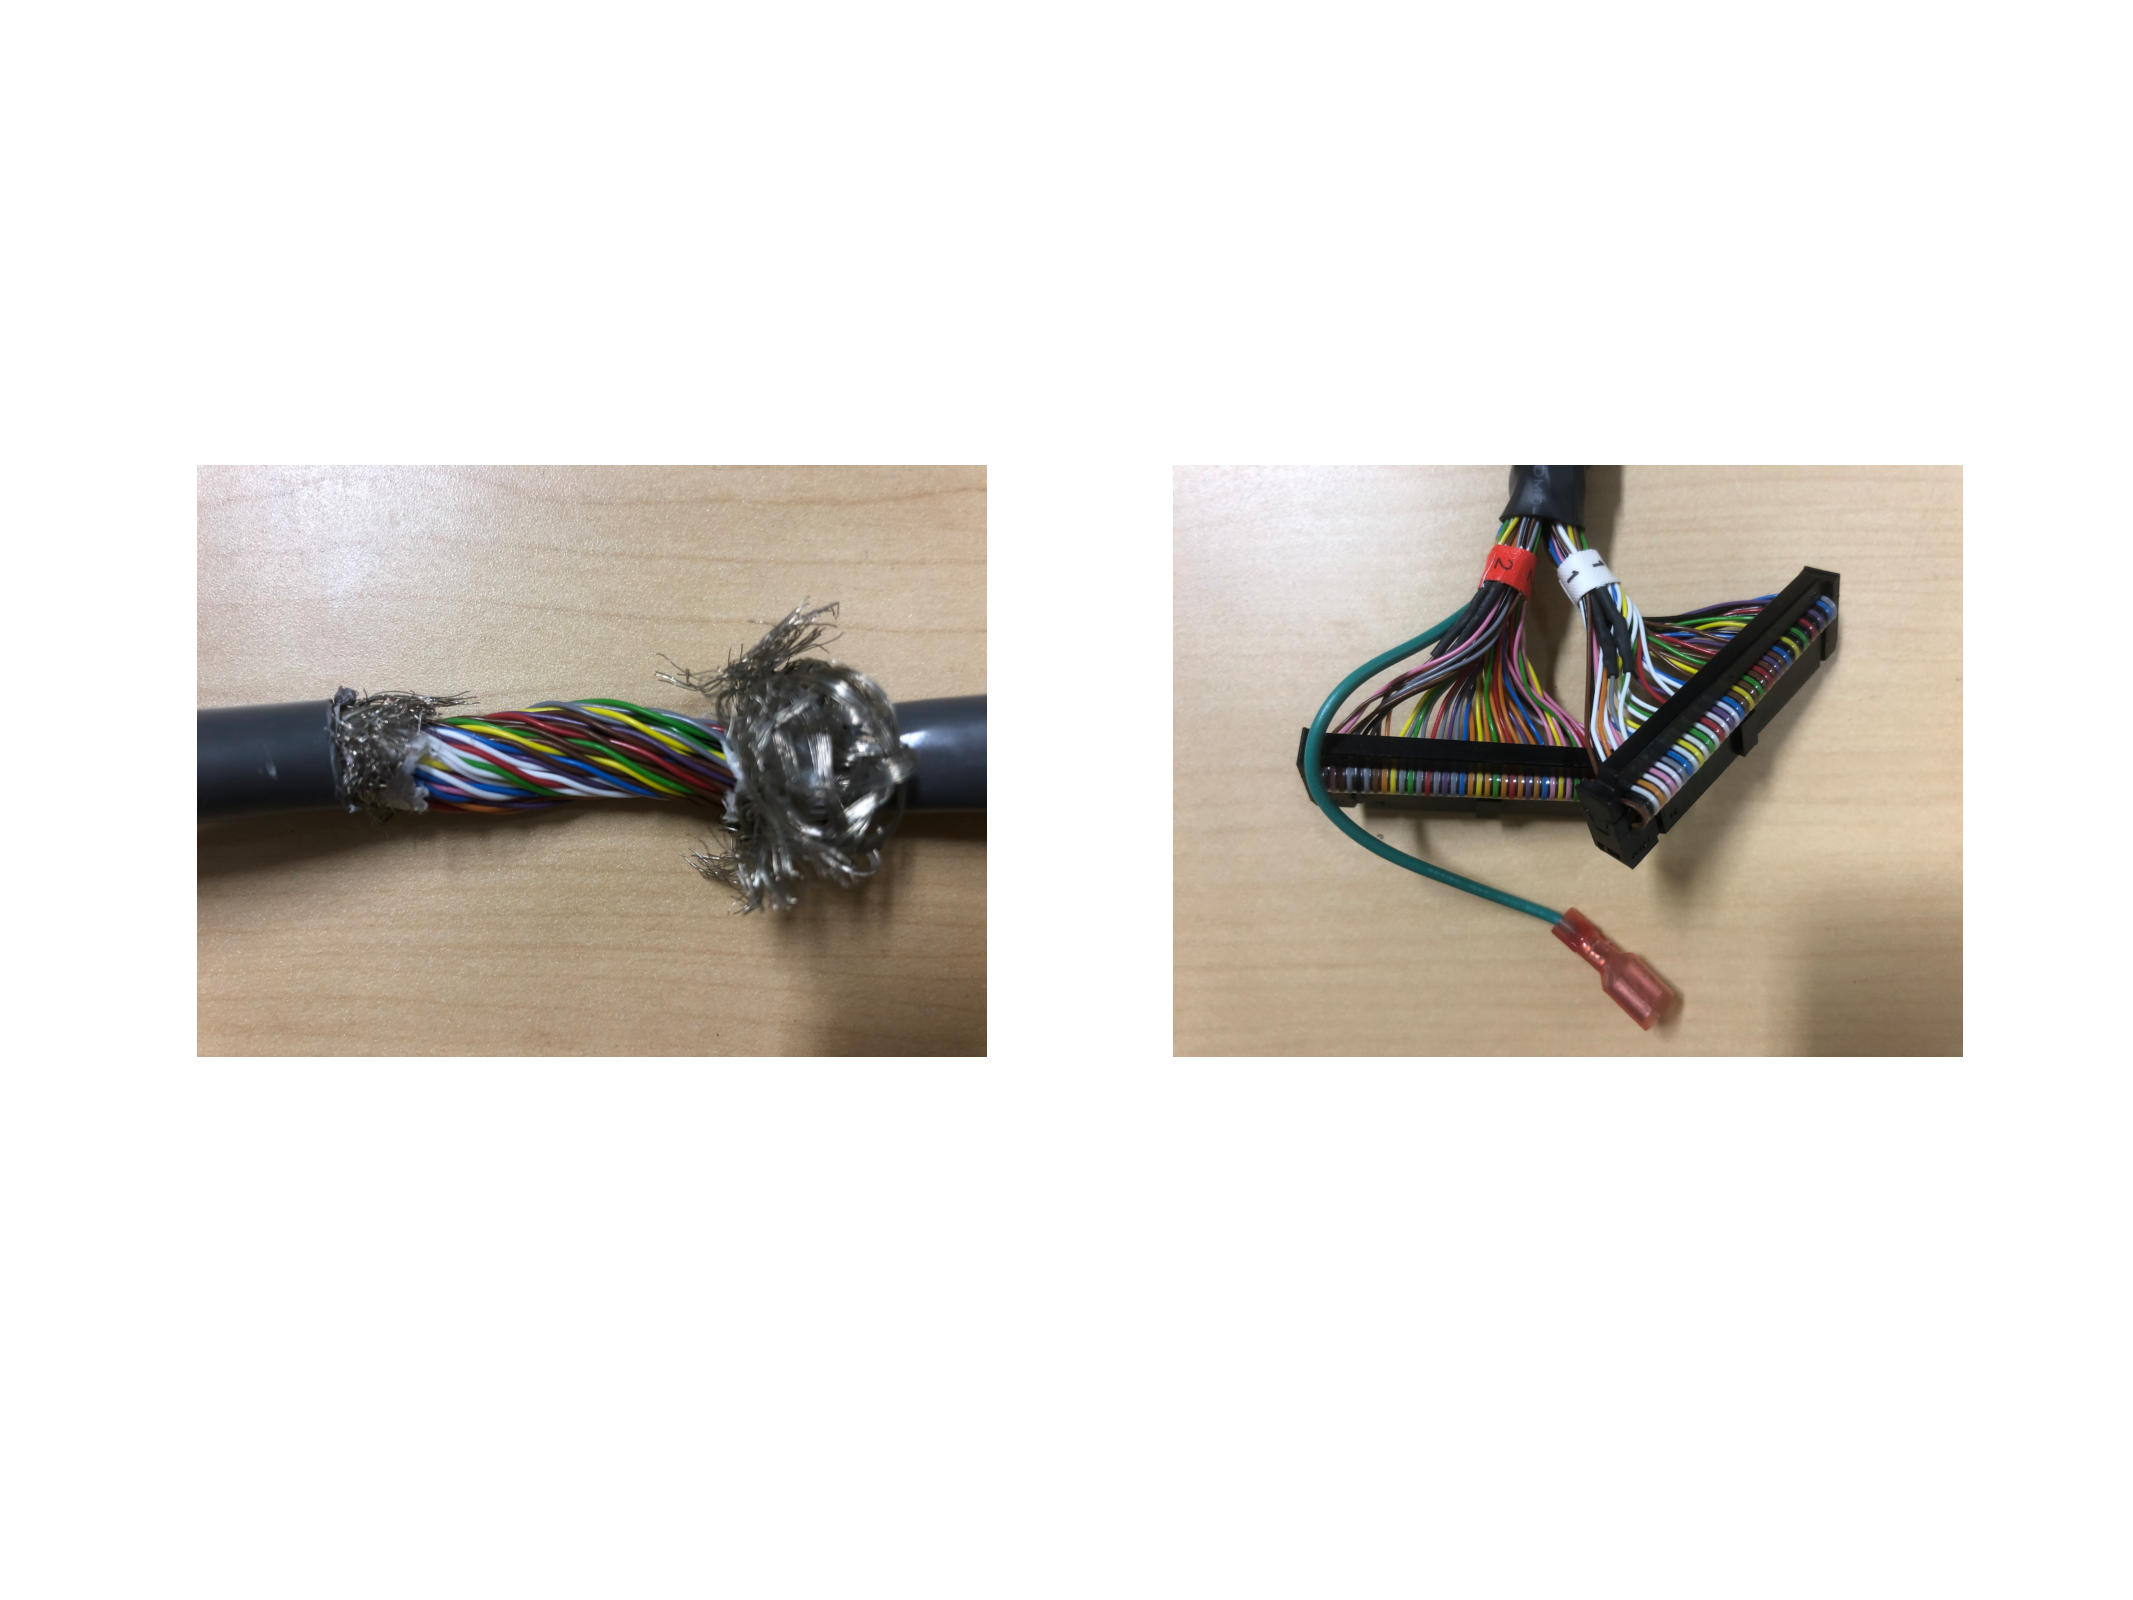
\includegraphics[width=\textwidth,page=1]{img/photo/twistphoto.pdf}
    \caption[ATLAS~実験で実際に使用されたシグナルケーブルの写真]{ATLAS~実験で実際に使用されたシグナルケーブルの写真。左図はケーブルの内部構造、右図は信号線の読み出し口。読み出しはケーブルの内側と外側でそれぞれまとめられて行われる。}
    \label{fig:twist00}
\end{figure}

\begin{figure}[H]
    \begin{minipage}{0.49\hsize}
    \centering   
    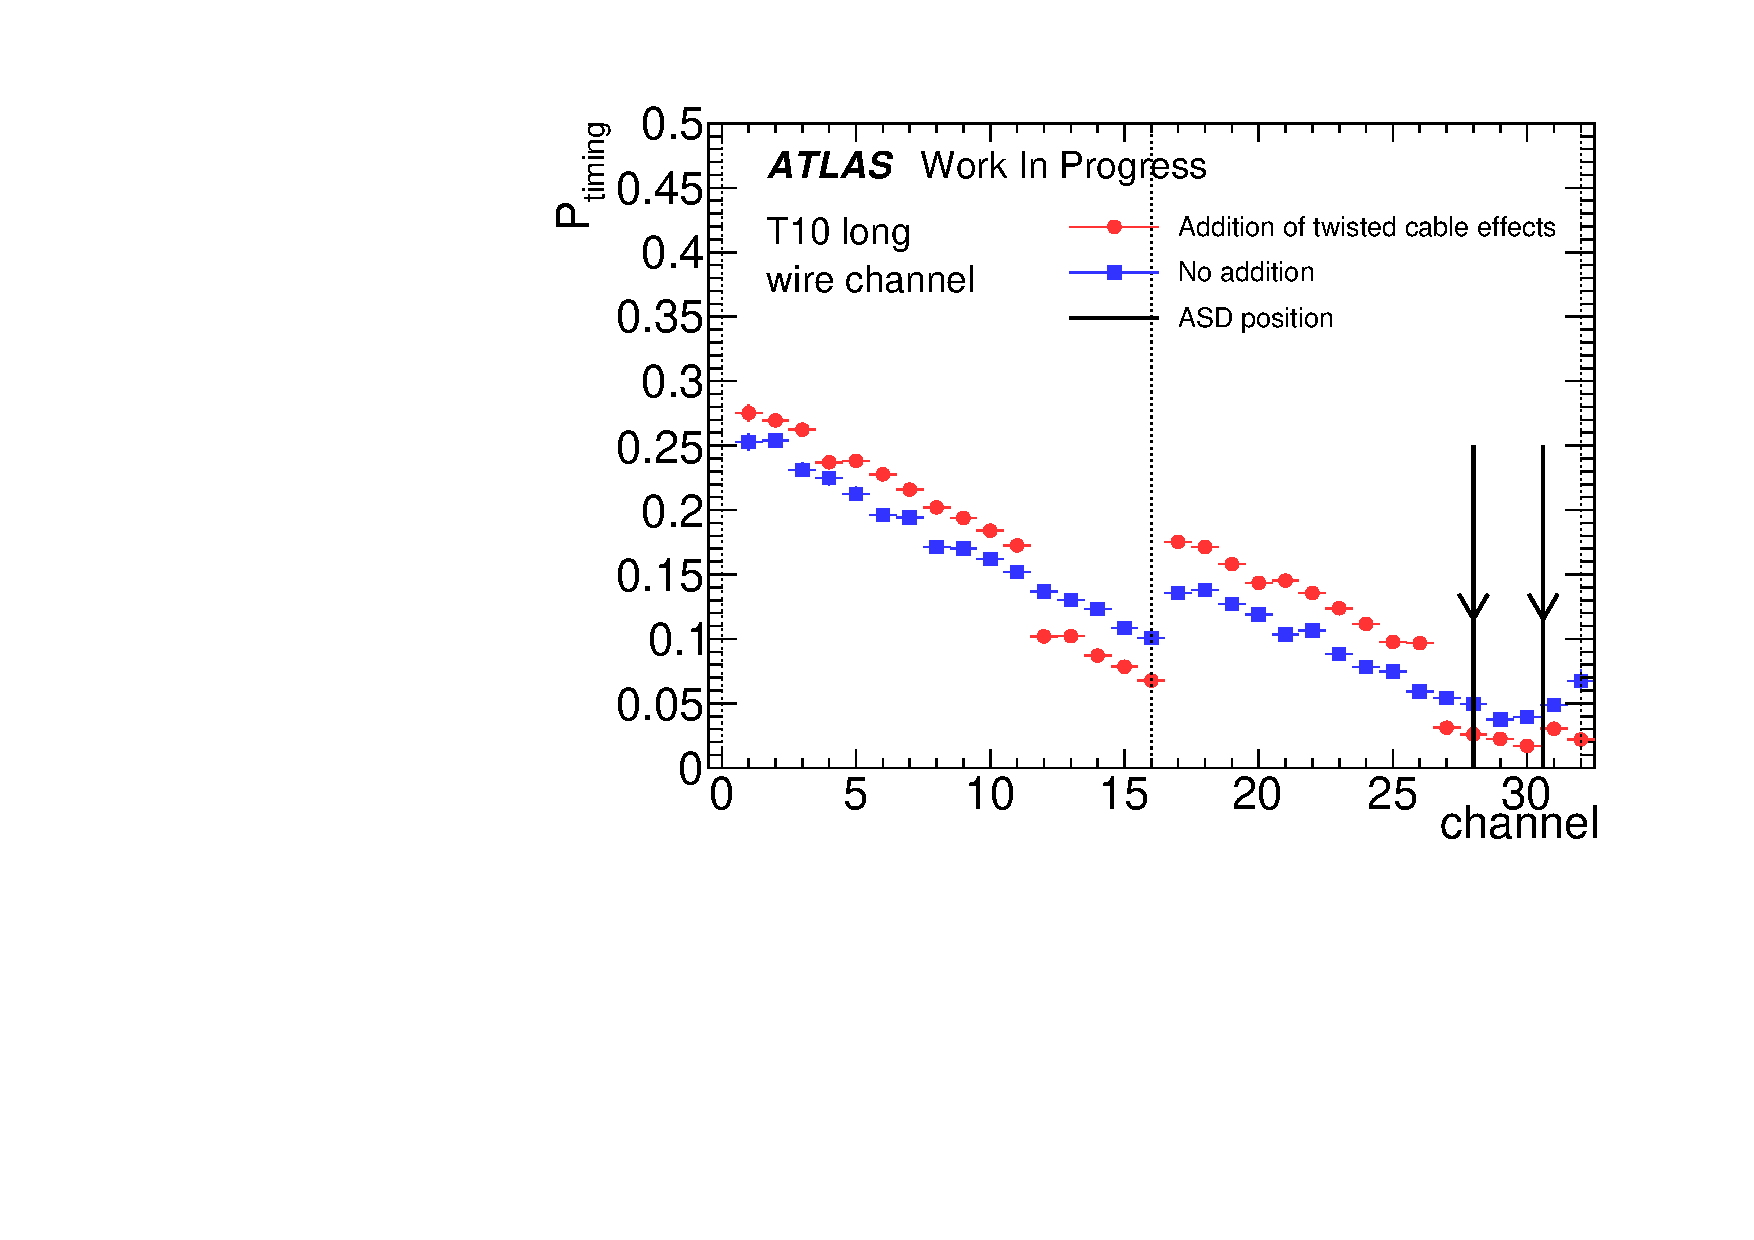
\includegraphics[width=\textwidth,page=1]{img/plot/twist.pdf}
    \subcaption{}
    \end{minipage}
    \begin{minipage}{0.49\hsize}
    \centering   
    \includegraphics[width=\textwidth,page=2]{img/plot/twist.pdf}
    \subcaption{}
    \end{minipage}
    \caption[ツイストケーブルの影響の実装によるタイミングの評価]{ツイストケーブルの影響の実装によるタイミングの評価。青は、ツイストケーブルの影響が未実装、赤は、ツイストケーブルの影響が実装されたシミュレーション。また両者には、ASD~までの信号伝搬の影響は実装済みである。(a)~FI~T10~チェンバー、wire~チャンネル。(b)~EI~T11~チェンバー、strip~チャンネル。}
    \label{fig:twist}
\end{figure}

\subsubsection{信号減衰による遅延時間の計算}
TGC~のセンサーにおいて信号が伝搬するに伴い信号の減衰が生じる~\cite{MT:04}。この効果により、センサーの長さに依存し信号検出までの遅延時間が発生する。
%実測した信号減衰の一例を\figref{fig:att2}に示した。信号が伝搬するケーブルの長さが長くなるにつれて、信号になまりが生じ信号の立ち上がりが緩やかになっていることがわかる。立ち上がりが緩やかになれば、閾値電圧を超えるタイミングも遅くなる。
遅延時間の関係を実測した結果が\figref{fig:att0}である。以上の結果から算出した\equref{eq:tdigit}をシミュレーションに新たに実装した。
\begin{align}
    信号減衰遅延 [{\rm{ns}}] =4.9×10^{-3}x^2+2.0×10^{-4}x
     \label{eq:delay}
\end{align}
$x [\rm{m}]$ は、ケーブル長を示している。

シミュレーションの実装前後における比較は\figref{fig:att}である。大きな差は見られないが、傾きに少しの変化があることが確認できる。

%\begin{figure}[H]
%    \centering   
%    \includegraphics[width=\textwidth,page=5]{img/slide/slide.pdf}
%    \caption[ケーブルの長さに依存した信号減衰の様子]{ケーブルの長さに依存した信号減衰の様子~\cite{URL:04}。下側は~PP~ASIC~が作ったテストパルスが~ASD~に届いた際の信号のアナログ出力を観測したもの。上側がテストパルスを受けて作られた~LVDS~がケーブルを伝搬し~PP~に届いた際の様子を観測したもの。ケーブル長が~2.8~m~の場合(左図)。ケーブル長が~47.3~m~の場合(右図)。}
%    \label{fig:att2}
%\end{figure}

\begin{figure}[H]
    \centering   
    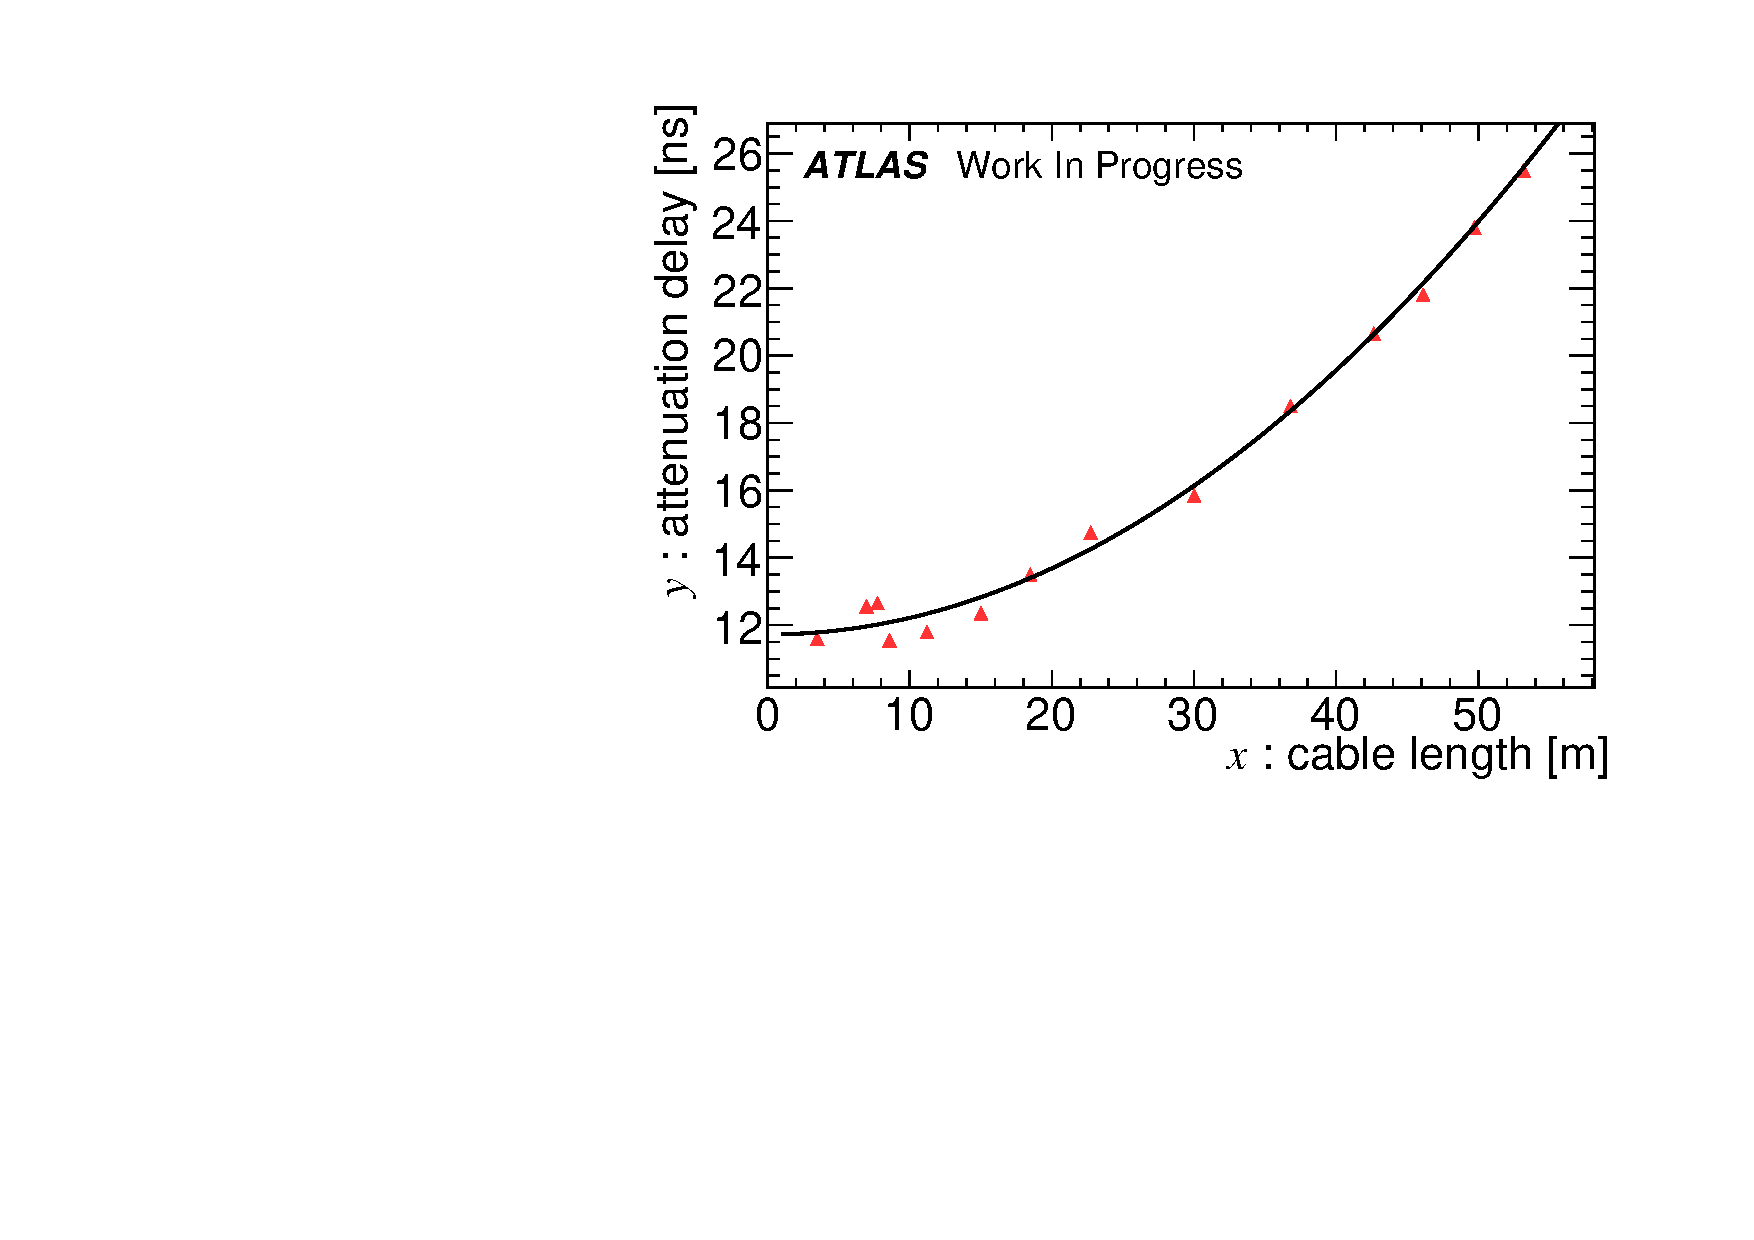
\includegraphics[width=0.7\textwidth,page=1]{img/plot/attk.pdf}
    \caption[信号減衰によるタイミングの遅れの実測値と近似式]{信号減衰によるタイミングの遅れの実測値と近似式~\cite{MT:04}。}
    \label{fig:att0}
\end{figure}

\begin{figure}[H]
    \centering   
    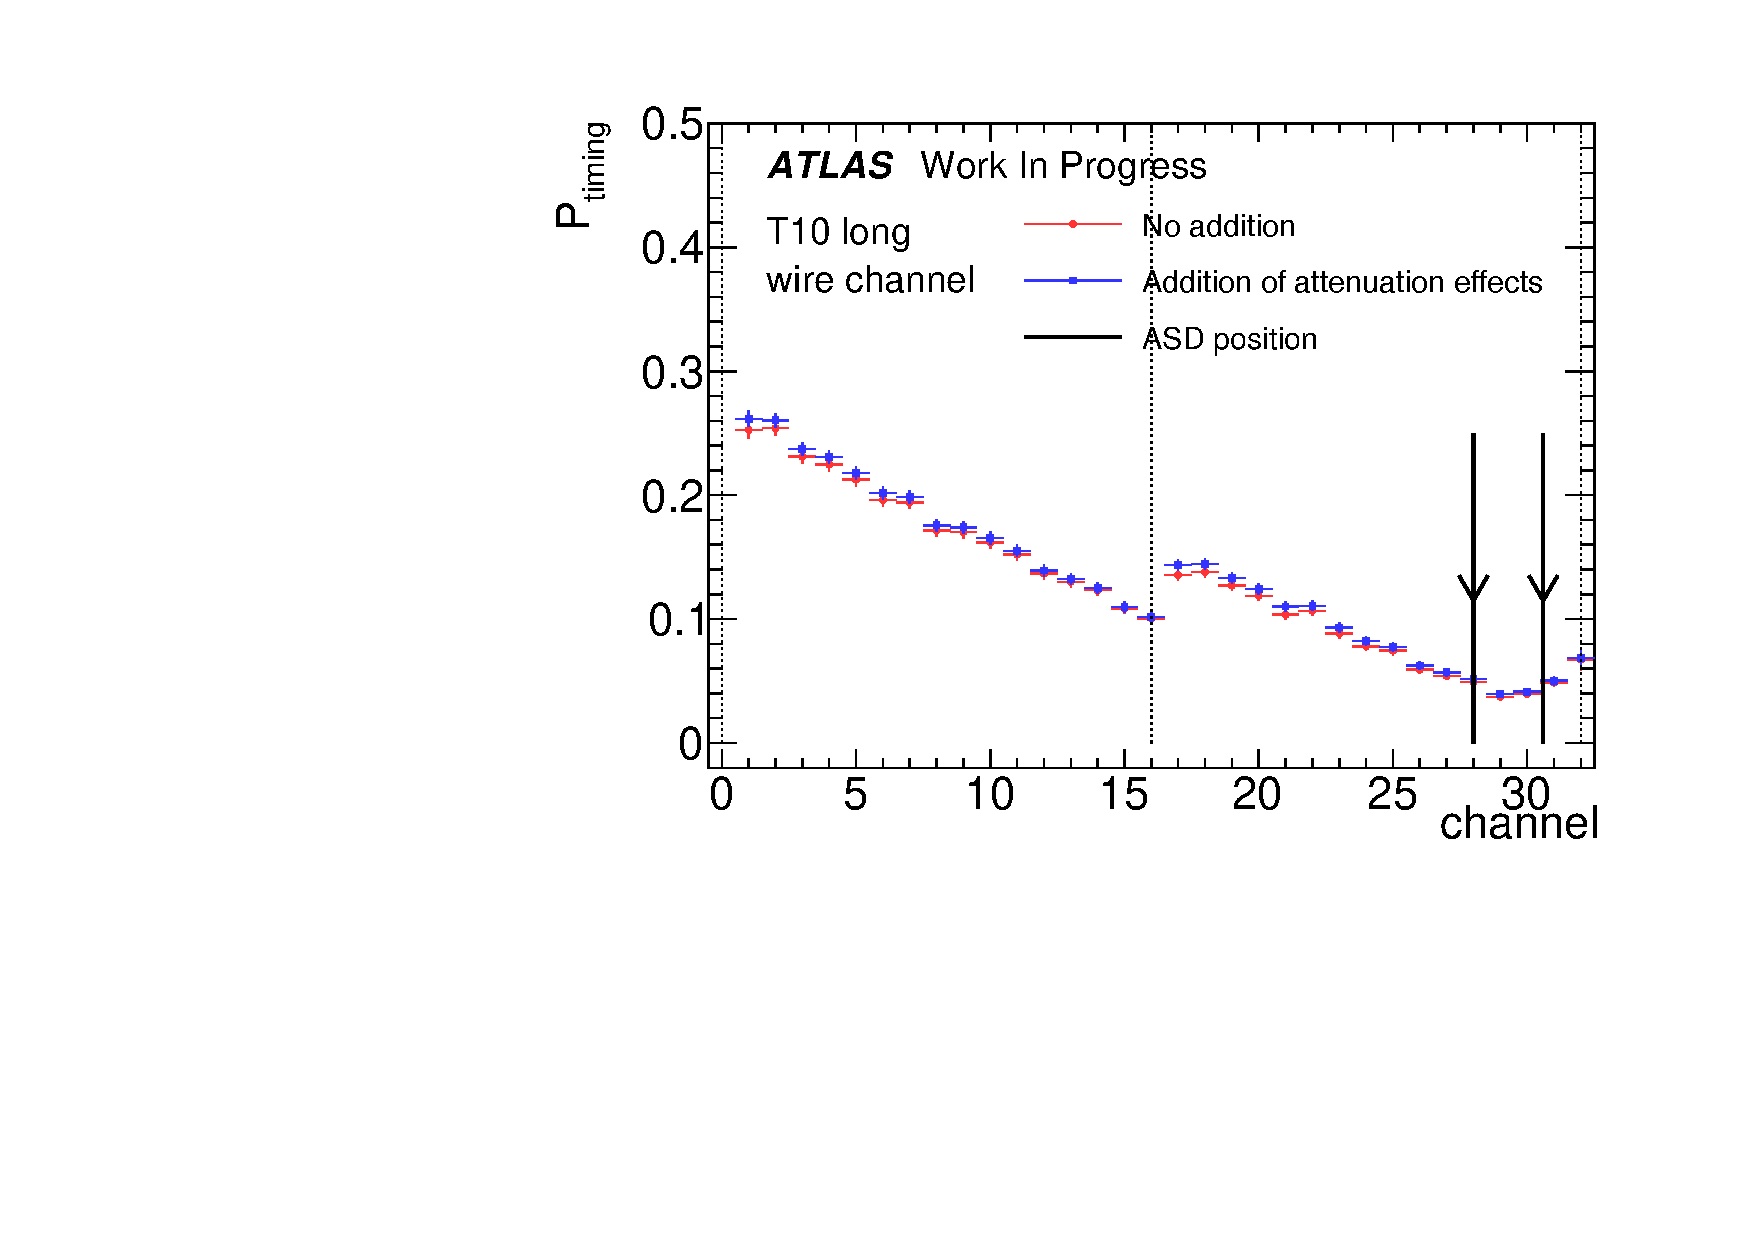
\includegraphics[width=0.7\textwidth,page=1]{img/plot/att.pdf}
    \caption[信号減衰の影響の実装によるタイミングの評価]{信号減衰の影響の実装によるタイミングの評価。赤は、信号減衰の影響が未実装、青は、信号減衰の影響が実装されたシミュレーション。また両者には、ASD~までの信号伝搬の影響は実装済みである。FI~T10~チェンバー、wire~チャンネル。}
    \label{fig:att}
\end{figure}

\subsubsection{データベースシステムの構築}
TGC デジタイゼーションでは、計算処理に必要な値を取得するためにテキストファイルからの値の読み込みが行われていた。テキストファイルによるデータ管理は、バージョン等による管理が不便であり非効率であった。
そこでテキストファイルベースの読み込み方法を刷新し、データベースを用いたシステムを新たに構築した。
以下ではデータベースとして実装した各計算処理について述べる。

\begin{itemize}
\item ASD position\\
ASD の配置は各チェンバーによって異なっている。ASD 配置の位置座標および対応するチャンネルをデータ化することで、センサーから ASD までの信号伝搬時間の計算が行えるようになる。
\item Time Offset\\
信号伝搬に対する遅延をかけタイミングをそろえるために、各チェンバーごとに時間のオフセットが用意されている。このオフセットが実験における遅延回路に相当する。
\item Cross Talk\\
粒子がセンサーに入射した場合、1 つのチャンネルに入力されるだけでなく、複数のチャンネルから読み取られる場合がある。このようなことが起きる確率は、粒子の入射角度、位置座標により決まっている。したがって、入射角度、位置座標によって決められた確率がデータに保存され計算が行われている。
\item Dead Chamber\\
実験においては、チェンバーの個々の特性の違いや故障等により電圧をかけず測定を行っていないチェンバーが存在する。これをデッドチェンバーと呼び、実験におけるデッドチェンバーの情報がデータベースに保存されている。
\item Energy Threshold\\
粒子のヒット信号の判定を行うために、信号に対する閾値電圧が実装されている。ヒット信号が閾値を超えると計算処理が行われるようになっている。閾値電圧は各チェンバーごとに設定することができる。
\item Time Jitter\\
ミューオンがガス中の電子を電離させ、電子が信号として検出されるまでには時間がかかる。検出までにかかる時間は、粒子の入射角度により変化し、確率的な揺らぎも生じる。入射角度ごとに対してシミュレーションに基づいたランダムな時間の揺らぎが計算される。
\end{itemize}

\subsection{TGC~検出器のタイミング較正}\label{subsec:cali}
\figref{fig:timingPlotBW}および\figref{fig:timingPlotSW}に\equref{eq:timing}のパラメータを使用したタイミングの評価を示す。改良前のモンテカルロシミュレーションにおいては、Run~2~の実験データを再現できておらず、理想的な状態としている~0~に近い位置でのプロットとなっていることがわかる。しかし、実際の実験データにおいては~ASD~の位置に依存したタイミング遅延がみられている。また、\figref{fig:timingPlotSW}ではツイストケーブルの影響によるタイミングの変化も確認できる。改良後のシミュレーションに関しては、Run~2~データにおけるこれらのタイミングの変化を詳細に再現していることがわかる。

以上に記したように、シミュレーションの改良を行ったことで、以前のシミュレーションと比べ実験データにおけるタイミングの変化を詳細に再現することに成功した。これにより、物理解析における系統的な誤差を削減し、よりデータに近い状態でのシミュレーションを用いた研究が可能となった。

また、ほかのチェンバーのタイミング較正についての詳細は、\appendixref{app:app1}に示した。

\begin{figure}[H]
	\begin{minipage}{0.49\hsize}
	\centering
	\includegraphics[width=\textwidth,page=10]{img/pdf5/master_timingplot_comp.pdf}
	\subcaption{}
	\end{minipage}
	\begin{minipage}{0.49\hsize}
	\centering
	\includegraphics[width=\textwidth,page=13]{img/pdf5/master_timingplot_comp.pdf}
	\subcaption{}
	\end{minipage}
	\caption[タイミングパラメータを用いた~TGC~BW~の評価]{タイミングパラメータを用いた~TGC~BW~の評価。橙色(■)、緑色(●)、青色(▲)はそれぞれRun 2 データ、改良後のシミュレーション、改良前のシミュレーションを表している。(a)~M1~T08~チェンバー、wire~チャンネル。(b)~M2~T02~チェンバー、strip チャンネル。}
	\label{fig:timingPlotBW}
\end{figure}

\begin{figure}[H]
	\begin{minipage}{0.49\hsize}
	\centering			
	\includegraphics[width=\textwidth,page=36]{img/pdf5/master_timingplot_comp.pdf}
	\subcaption{}
	\end{minipage}
	\begin{minipage}{0.49\hsize}
	\centering
	\includegraphics[width=\textwidth,page=37]{img/pdf5/master_timingplot_comp.pdf}
	\subcaption{}
	\end{minipage}
    \caption[タイミングパラメータを用いた~TGC~SW~の評価]{タイミングパラメータを用いた~TGC~SW~の評価。橙色(■)、緑色(●)、青色(▲)はそれぞれRun~2~データ、改良後のシミュレーション、改良前のシミュレーションを表している。(a)~FI~T10(Long) チェンバー、wire チャンネル、(b)~FI~T10(Long)チェンバー、strip チャンネル。}
	\label{fig:timingPlotSW}
\end{figure}

タイミング較正におけるステーションごとの数値結果を示す。\figref{tb:tunebcidM1}は M1、\figref{tb:tunebcidM2}は M2、\figref{tb:tunebcidM3}は M3、\figref{tb:tunebcidEIFI}は EIFI における 実験データおよびシミュレーションのバンチ判定の割合を示している。シミュレーションにおけるタイミング較正を行ったことで、実験データの分布に近づいていることがわかる。
\begin{table}[htb]
	\centering
	\begin{tabular}{c|c|c|c|c|c}\hline
	バンチ判定&前&前かつ基準&基準&基準かつ次&次 \\ \hline\hline
	実験データ(wire)& $0.04\%$ & $5.8\%$ & $92.7\%$ & $1.5\%$ & $1.4\%$ \\
	較正前(wire)& $0\%$ & $2.8\%$ & $97.2\%$ & $0.05\%$ & $0\%$ \\ 
	較正後(wire)& $0\%$ & $0\%$ & $96.1\%$ & $3.8\%$ & $0.1\%$ \\ \hline
	実験データ(strip)& $0\%$ & $38.6\%$ & $41.0\%$ & $19.8\%$ & $0.6\%$ \\
	較正前(strip)& $0\%$ & $37.8\%$ & $51.1\%$ & $11.1\%$ & $0\%$ \\
	較正後(strip)& $0\%$ & $19.6\%$ & $61.1\%$ & $19.3\%$ & $0\%$ \\
	\end{tabular}
	\caption{M1~ステーションにおけるバンチ判定分布割合}\label{tb:tunebcidM1}
\end{table}

\begin{table}[htb]
	\centering
	\begin{tabular}{c|c|c|c|c|c}\hline
	バンチ判定&前&前かつ基準&基準&基準かつ次&次 \\ \hline\hline
	実験データ(wire)& $0.06\%$ & $7.4\%$ & $88.8\%$ & $1.7\%$ & $0.7\%$ \\
	較正前(wire)& $0\%$ & $4.8\%$ & $95.1\%$ & $0.03\%$ & $0\%$ \\ 
	較正後(wire)& $0\%$ & $0\%$ & $97.1\%$ & $2.9\%$ & $0.04\%$ \\ \hline
	実験データ(strip)& $0\%$ & $40.2\%$ & $38.9\%$ & $19.8\%$ & $1.1\%$ \\
	較正前(strip)& $0\%$ & $36.5\%$ & $51.8\%$ & $11.7\%$ & $0\%$ \\
	較正後(strip)& $0\%$ & $14.7\%$ & $62.8\%$ & $22.5\%$ & $0\%$ \\
	\end{tabular}
	\caption{M2~ステーションにおけるバンチ判定分布割合}\label{tb:tunebcidM2}
\end{table}

\begin{table}[htb]
	\centering
	\begin{tabular}{c|c|c|c|c|c}\hline
	バンチ判定&前&前かつ基準&基準&基準かつ次&次 \\ \hline\hline
	実験データ(wire)& $0.08\%$ & $8.2\%$ & $88.1\%$ & $1.7\%$ & $0.7\%$ \\
	較正前(wire)& $0\%$ & $4.7\%$ & $95.3\%$ & $0.04\%$ & $0\%$ \\ 
	較正後(wire)& $0\%$ & $0\%$ & $97.1\%$ & $2.9\%$ & $0.03\%$ \\ \hline
	実験データ(strip)& $0.01\%$ & $43.8\%$ & $38.9\%$ & $16.7\%$ & $0.7\%$ \\
	較正前(strip)& $0\%$ & $39.1\%$ & $50.5\%$ & $10.4\%$ & $0\%$ \\
	較正後(strip)& $0\%$ & $18.0\%$ & $61.6\%$ & $20.4\%$ & $0\%$ \\
	\end{tabular}
	\caption{M3~ステーションにおけるバンチ判定分布割合}\label{tb:tunebcidM3}
\end{table}

\begin{table}[htb]
	\centering
	\begin{tabular}{c|c|c|c|c|c}\hline
	バンチ判定&前&前かつ基準&基準&基準かつ次&次 \\ \hline\hline
	実験データ(wire)& $0.04\%$ & $3.0\%$ & $73.2\%$ & $21.5\%$ & $2.2\%$ \\
	較正前(wire)& $0\%$ & $15.9\%$ & $84.0\%$ & $0.05\%$ & $0\%$ \\ 
	較正後(wire)& $0\%$ & $0\%$ & $73.8\%$ & $25.8\%$ & $0.4\%$ \\ \hline
	実験データ(strip)& $0.07\%$ & $54.3\%$ & $14.6\%$ & $23.7\%$ & $7.2\%$ \\
	較正前(strip)& $0\%$ & $65.7\%$ & $33.0\%$ & $1.3\%$ & $0\%$ \\
	較正後(strip)& $0\%$ & $6.5\%$ & $44.6\%$ & $48.9\%$ & $0\%$ \\
	\end{tabular}
	\caption{EIFI~ステーションにおけるバンチ判定分布割合}\label{tb:tunebcidEIFI}
\end{table}

%\subsection{エータ方向の依存性}
%\subsection{ファイ方向の依存性}
%\subsection{チェンバー毎の評価}
\subsection{ヒット効率の評価}
TGC~検出器におけるミューオンのヒット効率についての評価を行う。ヒット効率とは、TGC~検出器の~1~層においてどれだけの割合でヒットが検出されているかを表す量である。ヒット効率の定義式を\equref{eq:hit}に示す。
\begin{align}
    \frac{N^{\rm{Lyr2}}_{\rm{Hit\&muon}}~\&~N^{\rm{Lyr1}}_{\rm{Curr.\&Hit\&muon}}}{N^{\rm{Lyr2}}_{\rm{Hit\&muon}}} \label{eq:hit}
\end{align}
これは、TGC~検出器の~1~層目のレイヤーに対するヒット効率を示している。$N^{\rm{Lyr2}}_{\rm{Hit\&muon}}$~はミューオンのヒットがあった~2~層目のレイヤーに対する事象数を示している。また、$N^{\rm{Lyr1}}_{\rm{Curr.\&Hit\&muon}}$~は基準バンチにおけるミューオンのヒットがあった~1~層目のレイヤーに対する事象数を示している。2~層目に対しヒットを要求することで、1~層目でのヒット効率を算出することができる。

\figref{fig:hiteff}は~FI~T10~チェンバーにおける実験データとシミュレーションにおけるヒット効率を示した図である。Run~2~の実験データにおいてはヒット効率の位置依存性が観測できる。また、改良後のシミュレーションにおけるヒット効率においてもデータと同じように効率の位置依存性が再現されていることがわかる。これは、ASD~の配置によるタイミングの遅れが原因であると考えられる。T10~チェンバーにおいては\figref{fig:tgcT}で示したように~wire~における~ASD~の配置がジオメトリの関係上、端に寄った作りとなっている。この影響により、他のチェンバーと比べ~ASD~から遠い位置のチャンネルではタイミングの遅れが顕著になる。タイミングが遅れたことにより、適切なタイミングでヒットの処理が行われず、ASD~の位置に依存したヒット効率の低下がみられたのである。

以上の結果から、TGC~検出器におけるタイミング調整が、ヒット効率へ影響を与えることを示唆することができた。

\begin{figure}[H]
	\begin{minipage}{0.49\hsize}
	\centering
	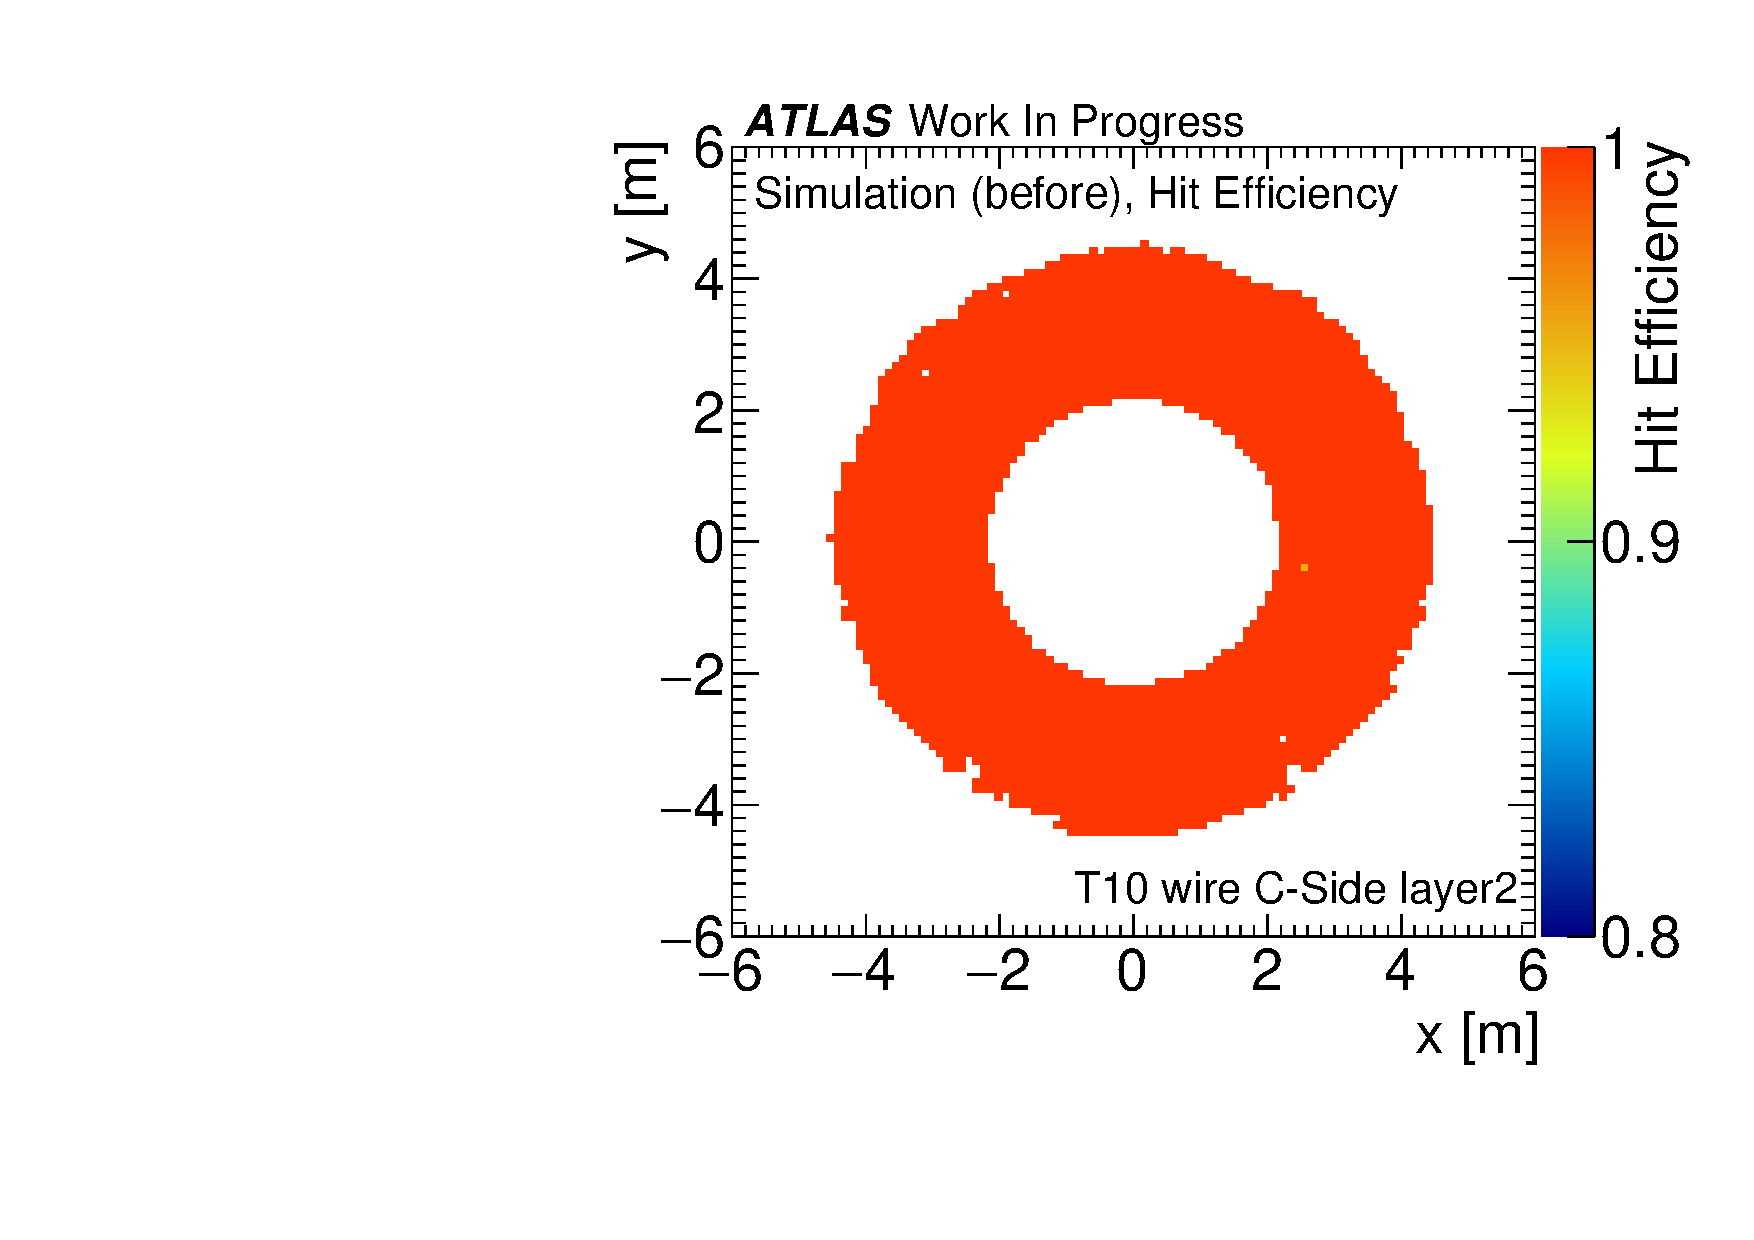
\includegraphics[width=\textwidth,page=1]{img/plot/hit_eff_orin.pdf}
	\subcaption{}
	\end{minipage}
	\begin{minipage}{0.49\hsize}
	\centering
	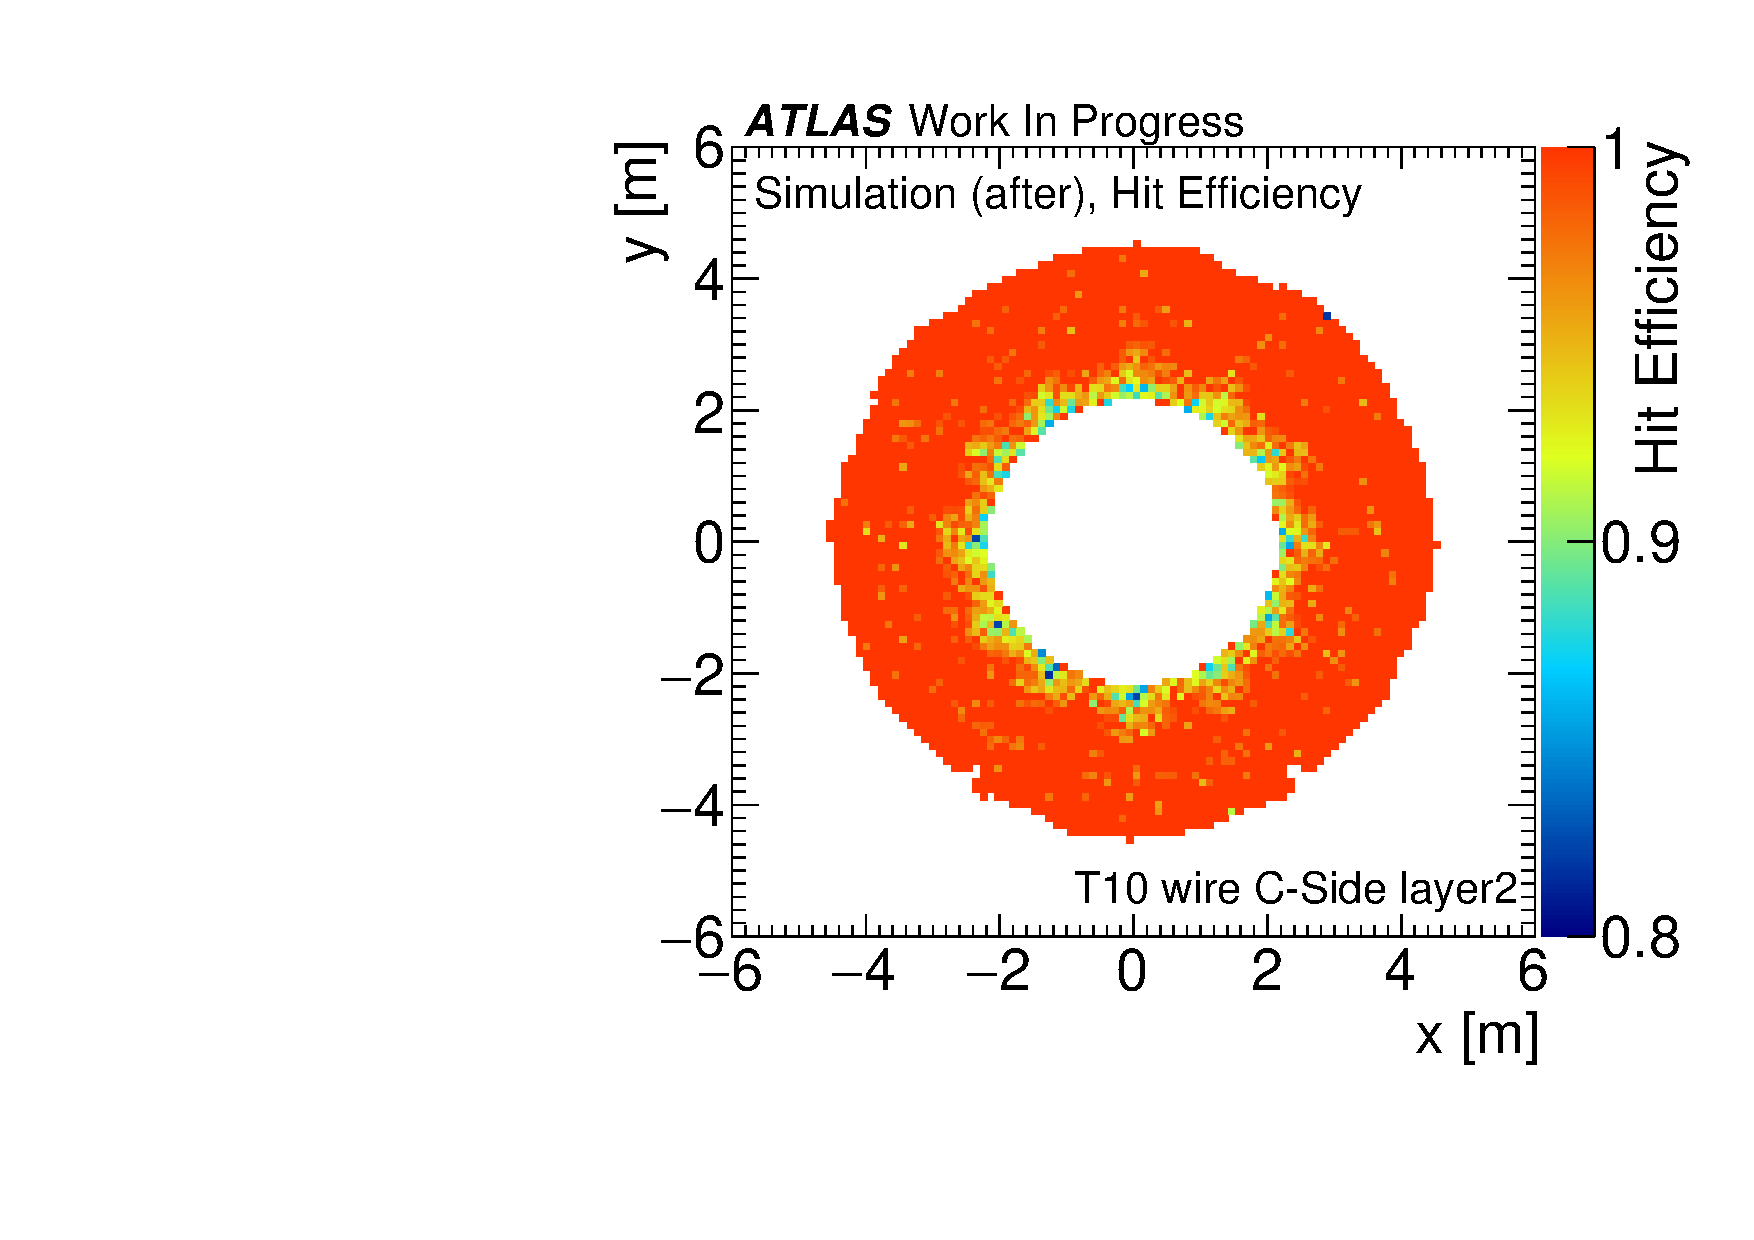
\includegraphics[width=\textwidth,page=1]{img/plot/hit_eff_tune.pdf}
	\subcaption{}
	\end{minipage}\\
	\begin{minipage}{0.99\hsize}
	\centering
	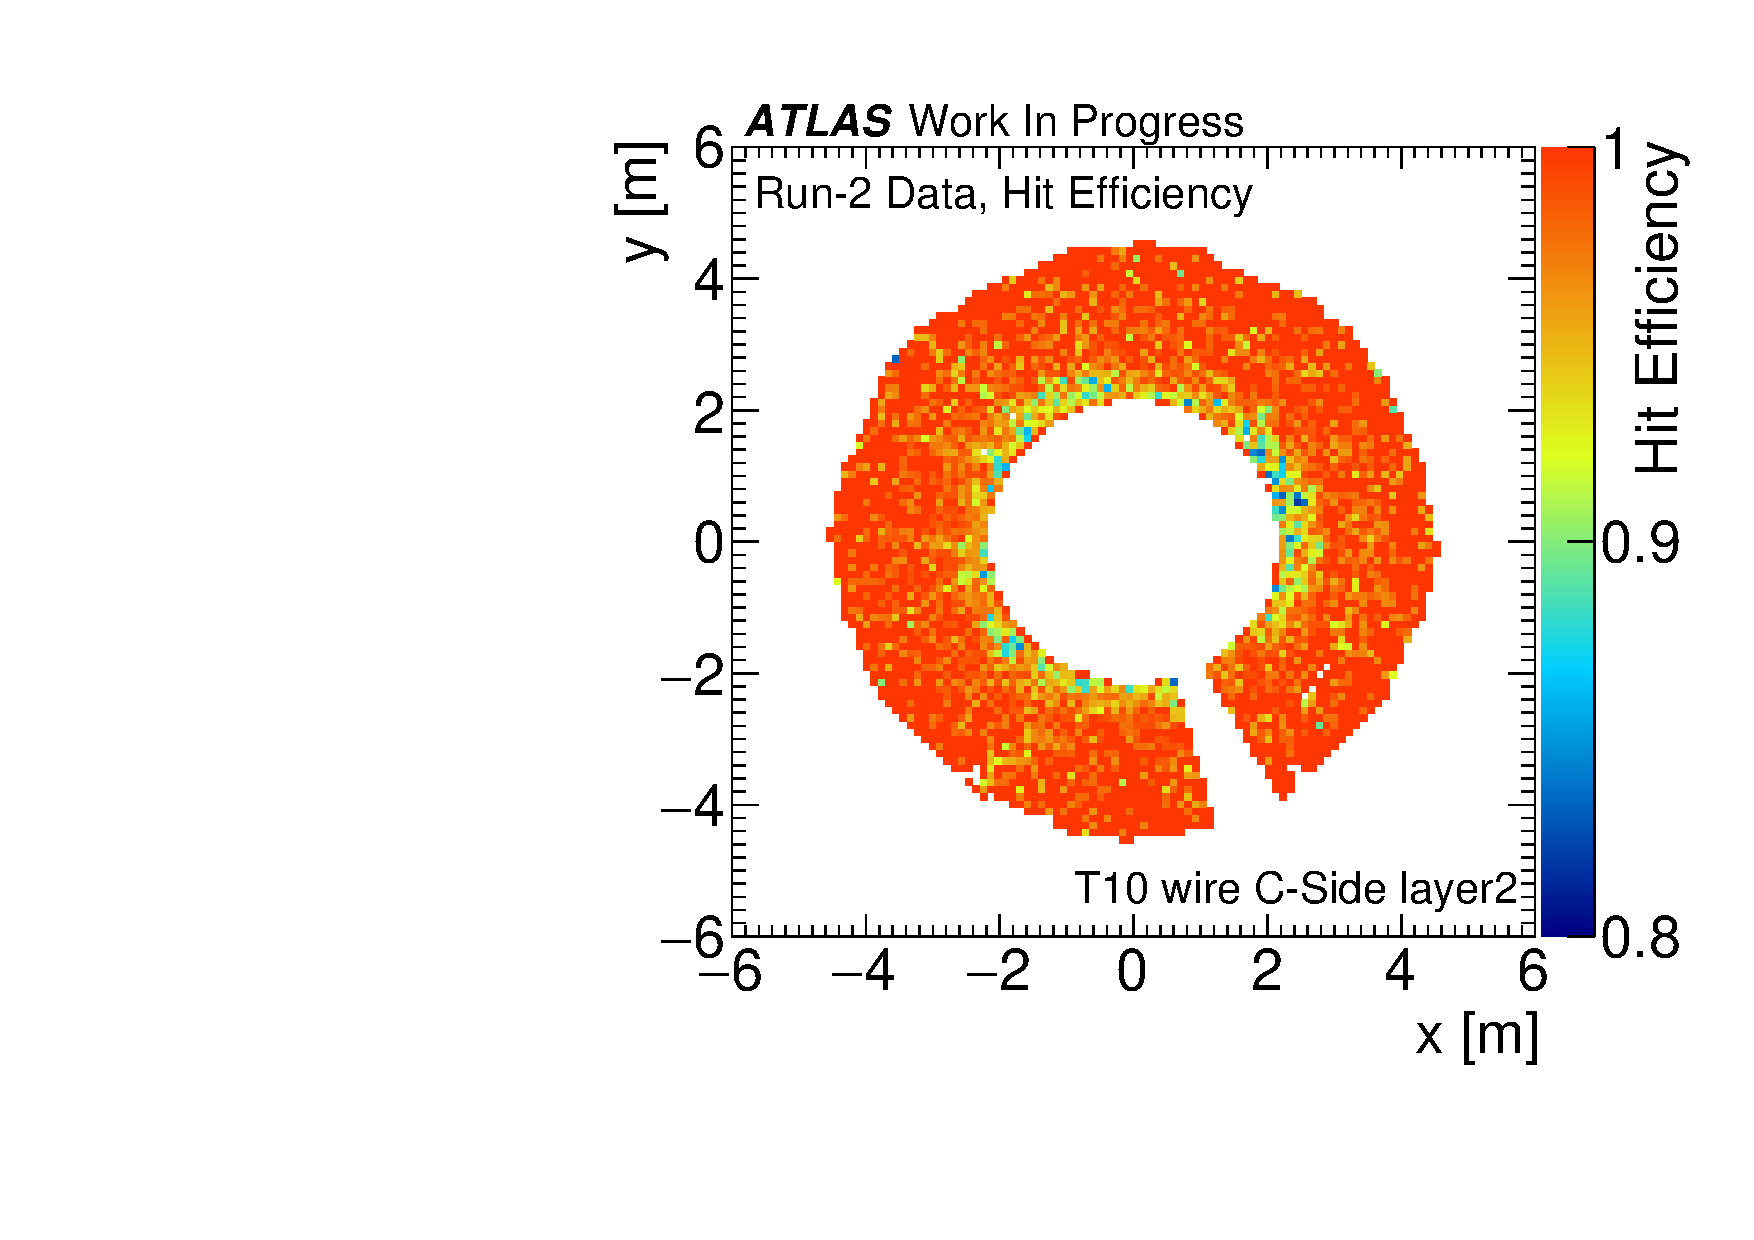
\includegraphics[width=0.49\textwidth,page=1]{img/plot/hit_eff_data.pdf}
	\subcaption{}
	\end{minipage}
	\caption[データとシミュレーションにおけるヒット効率の比較]{データとシミュレーションにおけるヒット効率の比較。FI~T10~チェンバー、C-Side、レイヤー2~におけるヒット効率。(a)~タイミング較正前のシミュレーション。(b)~タイミング較正後のシミュレーション。(c)~Run~2~の実験データ。較正後のシミュレーションが実験データの位置依存性を再現している。}
	\label{fig:hiteff}
\end{figure}

\section{Run~3~に向けた~TGC~検出器の性能改善}
本章では~TGC~検出器のタイミングについての詳細な検証およびシミュレーションの改良を行った結果を示した。シミュレーションの改良により~Run~2~の結果を詳細に再現することに成功した。また~TGC~検出器のヒット効率における位置依存性をバンチ判定のタイミング検証により評価を行い、改善法を示した。本節では~Run~3~に向けた~TGC~検出器の性能改善について言及する。

\subsection{タイミング遅延の改善}
前節より、FI~T10~チェンバーにおいてタイミングの遅れによるヒット効率の非効率な位置依存性がみられることがわかった。このヒット効率の低下を改善するために~T10~チェンバーにおける遅延パラメータの改良を提案する。\figref{fig:fitune}は、シミュレーションにおけるタイミング較正を行った上で、遅延パラメータを~1~ns~おきに変化させることでタイミング判定がどのように変化するかを表した図である。

タイミングの最適化を行う上で、もっとも重要なことはバンチ判定が、前のバンチあるいは次のバンチに判定されないようにし、光速のミューオンが基準バンチで最大限に読み出されるような調整を行うことである。\figref{fig:fitune}において以上のような条件を満たすには、もともとの実装状態に対し~$4~-~5~\rm{ns}$~の遅延を加えることが最適であると考えられる。実験においては、PP~ASIC~での遅延を~$4~-~5~\rm{ns}$~増加させることに対応する。
FI~T10~チェンバーにおける以上のタイミング調整は、実験に使用されるオンラインパラメータへの実装を行った。
\begin{figure}[H]
    \centering   
    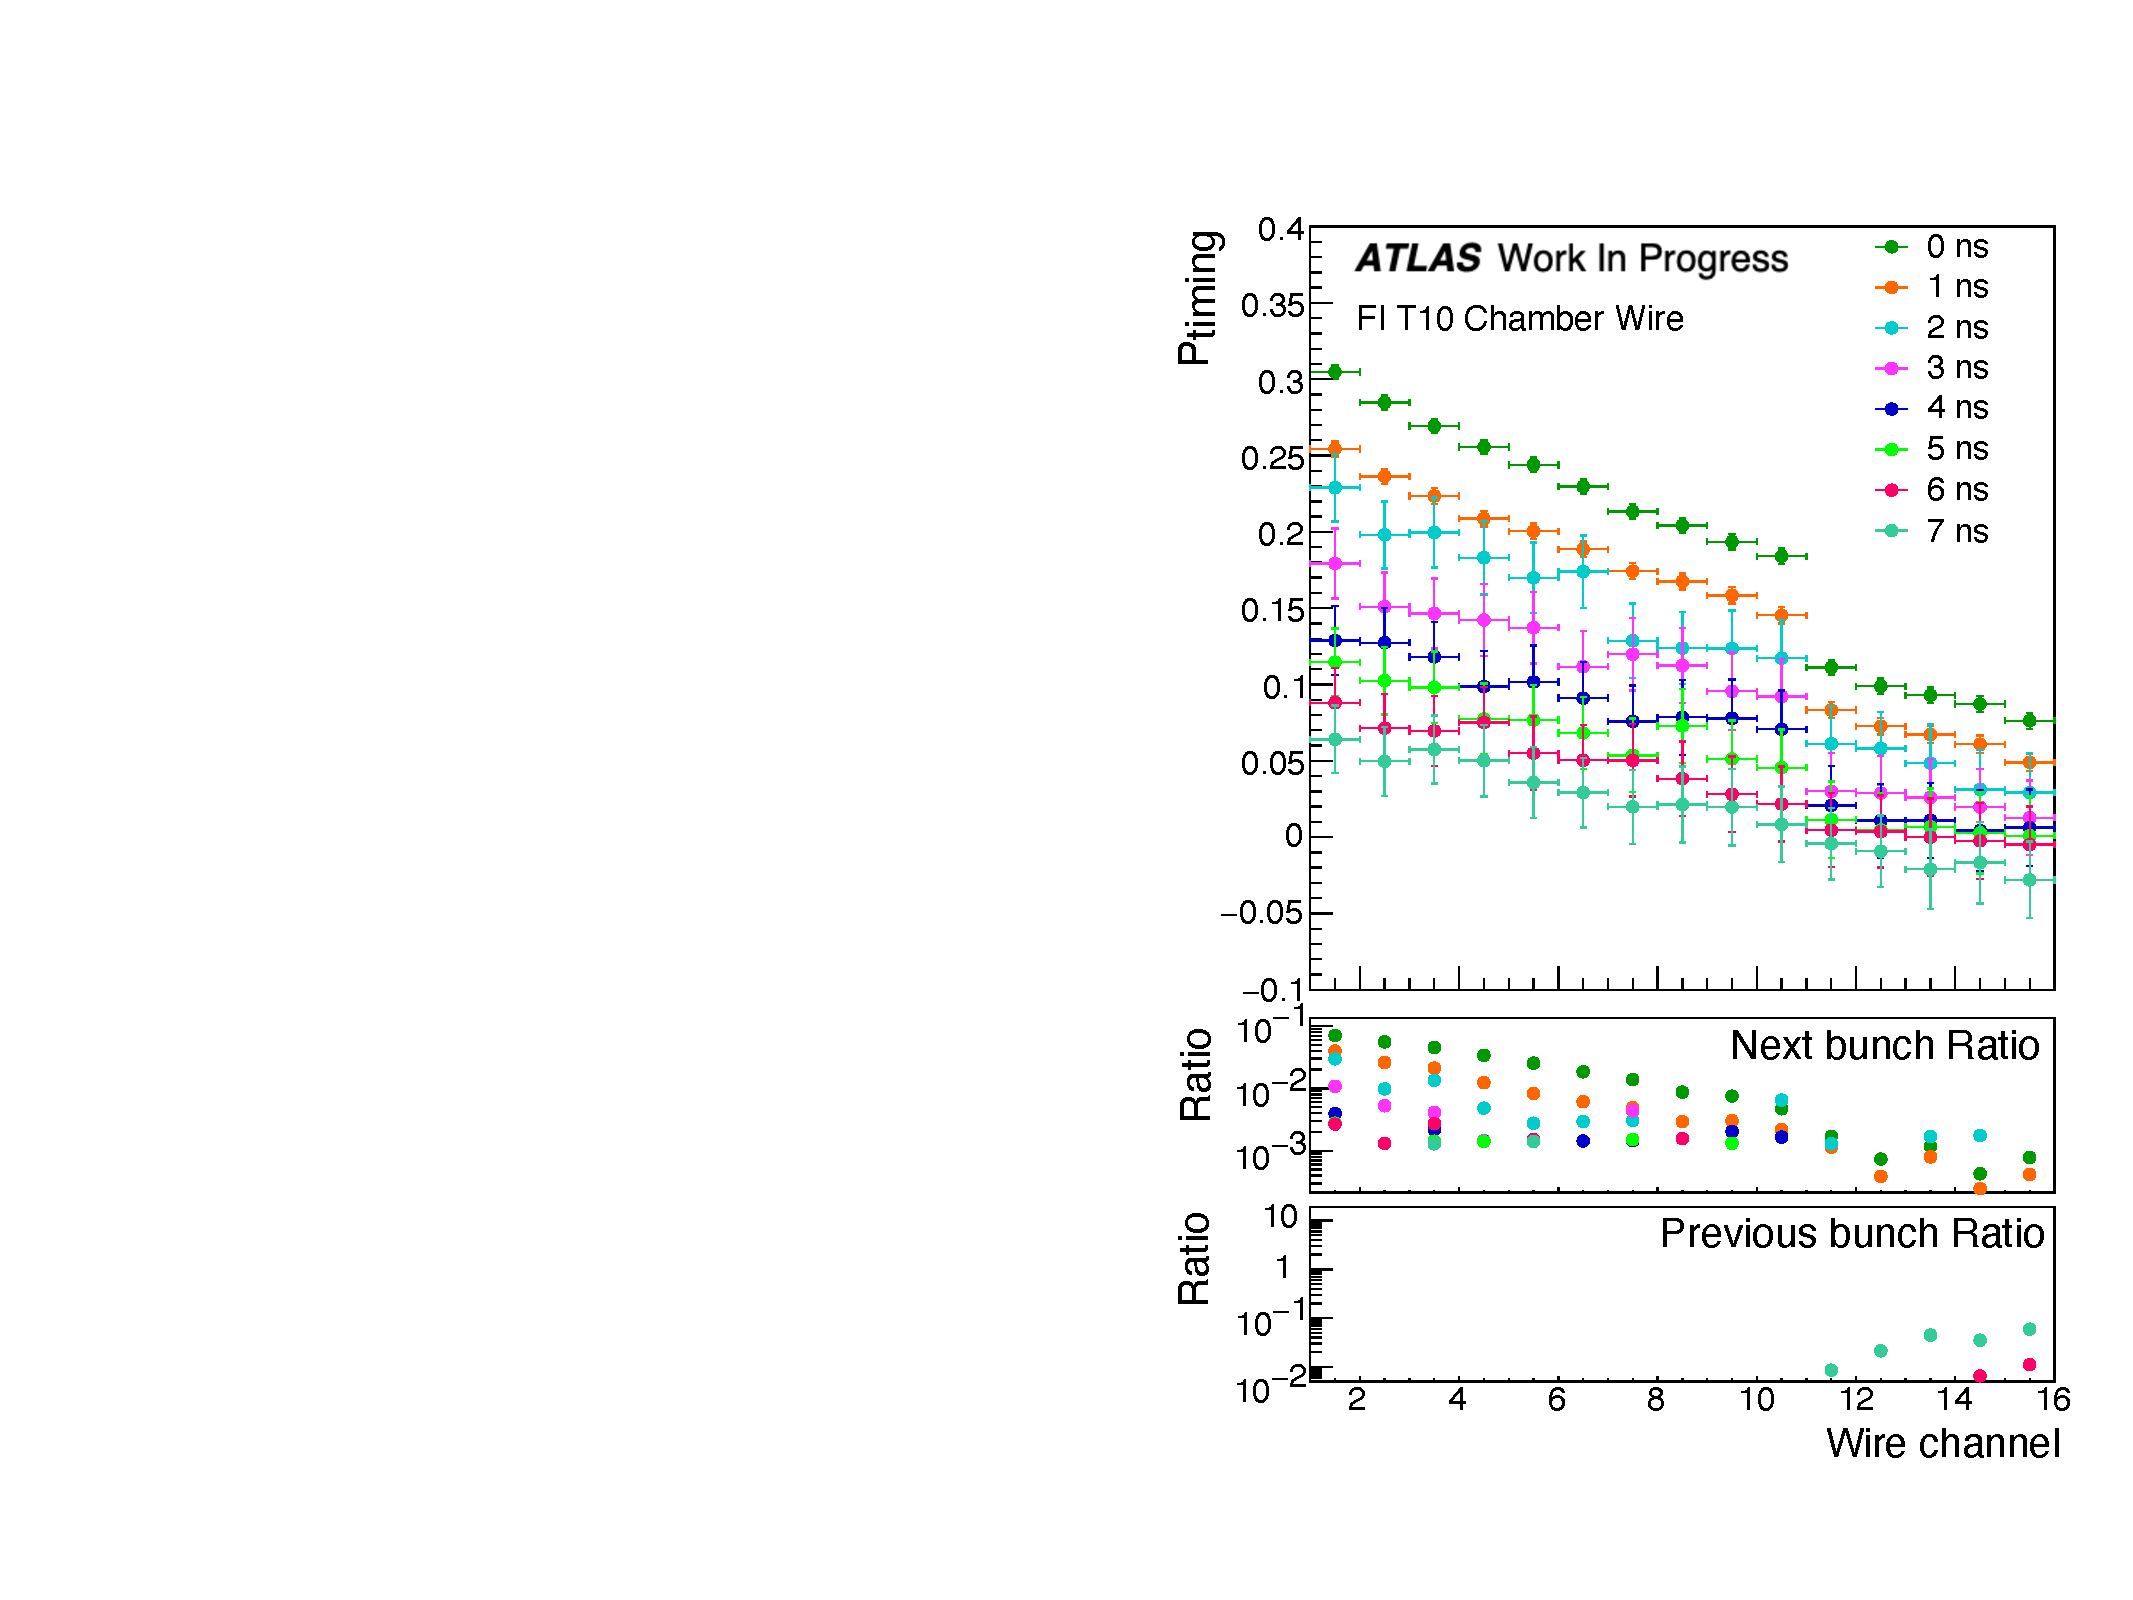
\includegraphics[width=0.8\textwidth,page=1]{img/plot/FItune.pdf}
    \caption[FI T10 チェンバーにおける遅延パラメータの調整]{FI~T10~チェンバーにおける遅延パラメータの調整。タイミング較正後のシミュレーション(0~ns)から、遅延パラメータを~1~ns~ずつ遅らせた場合のふるまいを示している。}
    \label{fig:fitune}
\end{figure}

\subsection{Run~3~に向けたタイミング調整}
Run~3~が開始されれば、大幅なアップグレードに伴い、改めてタイミング調整が行われることになる。Run~3~初期の段階では遅延回路におけるパラメータを変化させながら、タイミングのスキャンを実行することで~TGC~検出器におけるタイミング設定の検証を行う。実行の際には、本研究におけるタイミング評価方法を用いることで、遅延パラメータとバンチ判定の関係を容易に評価することが可能である。また精密な実装を行ったモンテカルロシミュレーションとの比較を行えば、PP~ASIC~等での遅延パラメータによる影響の詳細な評価を行える。
本研究により行ったタイミング較正の結果より、Run~3~の開始に向けた改善点とタイミングの評価方法について示唆することができた。
